\documentclass[11pt]{article}
\usepackage{amsmath,amssymb,amsthm}
\usepackage{graphicx}
\usepackage[margin=1in]{geometry}
\usepackage[table]{xcolor}
\usepackage{csvsimple}
\usepackage{enumitem}
\usepackage{float}
\usepackage{caption}
\usepackage{longtable}
\usepackage{hyperref}
\captionsetup[table]{justification=raggedright,singlelinecheck=off,labelfont=bf}
\usepackage{subcaption}
\restylefloat{table}
\usepackage{fancyhdr}
\setlength{\parindent}{0pt}
\setlength{\parskip}{5pt plus 1pt}
\setlength{\headheight}{13.6pt}
\newcommand\question[2]{\vspace{.25in}\hrule\textbf{#1: #2}\vspace{.5em}\hrule\vspace{.10in}}
\renewcommand\part[1]{\vspace{.10in}\textbf{(#1)}}
\newcommand\algorithm{\vspace{.10in}\textbf{Algorithm: }}
\newcommand\correctness{\vspace{.10in}\textbf{Correctness: }}
\newcommand\runtime{\vspace{.10in}\textbf{Running time: }}
\pagestyle{fancyplain}
\lhead{\textbf{\NAME\ (\ANDREWID)}}
\rhead{Page \thepage}
\begin{document}


%Section A==============Change the values below to match your information==================
\newcommand\NAME{Turaga}  % your name
\newcommand\ANDREWID{nturaga1@jhmi.edu}     % your andrew id
%\newcommand\HWNUM{1}              % the homework number

\title{Differential Methylation Analysis of H460 Parent and H460 Knock-in cell lines on 2.1M Nimblegen Array}
\author{Nitesh Turaga}
\maketitle



To perform differential methylation analysis of H460 knock-in and H460 parent cell lines.The data was generated by Nimblegen 2.1M microarrays. Raw data are in the form of images (TIF files). Data set included total of 6 samples, 3 for each cell line (H460 knock-in and H460 parent). Array images were processed with DEVA-v1.2 (Nimblegen software for automated feature extraction and data analysis). The TIF files were converted to {\bf XYS} files for analysis. These files report the, {\bf X} - coordinate of the feature on the image, {\bf Y}-coordinate of the feature on the image, and the {\bf S}ignal - the flourescence intensity of the pixels that make the feature. The TIF files were also processed with DEVA using the DNA methylation work flow to identify peaks for each sample.

%%%%%%%%%%%%%%%%%%%%%%%%%% 
\section*{Preliminary Assessments}
%%%%%%%%%%%%%%%%%%%%%%%%%%


General QC-analyses brought to light that the signal intensities and local enrichment at methylated sites were not large. The data quality was assessed by looking at the Enriched channel in the MeDIP array, where we expect every probe to have a signal. Since, the enriched channel has methylated DNA, a successful hybridization would indicate a signal. The array signal is calculated as the average percentile rank of the signal probes among the background probes. The score ranges between 0 to 100, where 100 indicates the ideal scenario or perfect hybridization. This quality score is calculated before any kind of normalization is done on the arrays.


\captionof{table}{Array quality scores}
\begin{table}[H]
    \begin{tabular}{|l|l|l|}
    \hline
    Sample ID                        & Status       & Quality Score     \\ \hline
    542586A01\_Slot9\_2012-07-24\_H460 & H460\_parent & 59.6  \\ \hline
    542737A01\_Slot13\_2012-07-24\_H460 & H460\_parent & 64.4  \\ \hline
    542857A01\_Slot18\_2012-07-24\_H460 & H460\_parent & 69.8  \\ \hline
	542671A01\_Slot6\_2012-07-24\_H460 & H460\_knockin & 71.2  \\ \hline
    542654A01\_Slot9\_2012-07-25\_H460 & H460\_knockin & 74.9  \\ \hline    
    542707A01\_Slot12\_2012-07-25\_H460 & H460\_knockin & 76.5   \\ \hline
    \end{tabular}

\end{table}

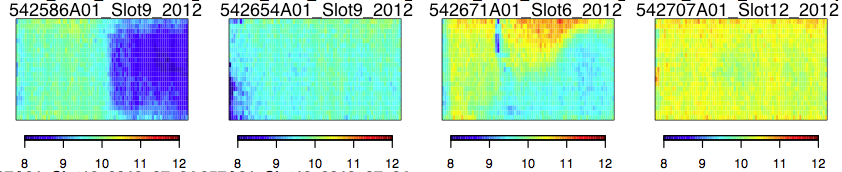
\includegraphics[scale=0.5]{qcImage1.png}

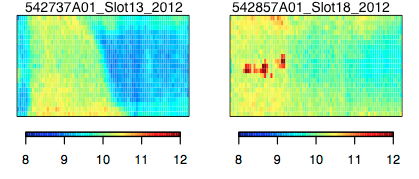
\includegraphics[scale=0.5]{qcImage2.png}


As we can in Table 1, the quality score of the H460 Parent arrays are pretty low.

%%%%%%%%%%%%%%%%%%%%%%%%%% 
\section*{The CHARM Algorithm}
%%%%%%%%%%%%%%%%%%%%%%%%%%

%Array quality scores were generated with the  Bioconductor {\tt charm - package}, and data quality was checked using the $Enriched$ channel. Four of the six arrays show a large standard deviation in the signal strenth and seem to have a problem in hybridization.
%
%To estimate the DNA methylation values, the background signal is removed before computing the log-ratios. A within sample normalization method - {\bf loess} is used, and then a between array normalization - quantile  is used. The control probes which are the non-CpG probes are excluded. This provides us a probe-level estimate of DNA methylation from the 2.1M oligonucliotide microarray.
%

%CHARM is specifically designed to maximize the number of assayed CpGs. This improves the detection strategy because it facilitates a smoothing strategy and assays many more CpGs.

The basic measurement used to quantify methylation is the log-ratio of the intensities observed in the treated and control channels. To detect methylated regions in CHARM, the M-values were normalized and processed using genome-weighted smoothing. The normalization method uses genome sequence information and knowledge of select pseudo-housekeeping probes for which one can assume M = 0. Loess is applied to the pseudo-housekeeping genes, to correct M-values for all probes. To obtain a smoothed M-value at any given genomic location, average all the M-values that were within a prespecified distance from the location in question. The interval providing the values that are averaged is referred to as the “smoothing window” and its length is referred to as the “window size.” \href{http://www.ncbi.nlm.nih.gov/pmc/articles/PMC2336799/}{(5)} \\

After estimating the DNA methylation in terms of percentage methylation, we use the regression based DMR-finding approach after correcting for batch effects. No DMRs were found using this method.


%%%%%%%%%%%%%%%%%%%%%%%%%%% 
%\section*{The Bumphunter Algorithm}
%%%%%%%%%%%%%%%%%%%%%%%%%%%
%
%
%Bumphunter used to estimate regions for which the genomic profile deviates from a baseline value(cut off). It is implemented to detect differntially methylated genomic regions between two populations. It is also a regression based approach.It reports the result, with a table of candidate differentially methylated regions and the corresponding annotation for wach region.

%
%{\bf Analysis using Bumphunter}
%
%
%\begin{enumerate}
%
%\item Run  1
%
%Initially ran {\tt bumphunter} on the data, with cutoff value 1.0, this failed to find any bumps. The sensitivity of the cutoff was not enough to catch any DMRs in the sample set. Bumphunter is better used for large sample sets, for better performance. 
%
%
%\item Run  2
%
%Bumphunter, with the inbuilt argument to pickCutoff was run. The cutoff chosen by bumphunter was at 0.41, bumps found 28206. The number of DMRs/bumps of length greater than four is 0. This result is not useful for analysis as the length of the DMRs are too small.
%
%%bumps.rda file attached. 
%
%The distribution of the length of DMRs found, is shown below. Most of them are single CpG sites of length 1. This does not work for a significant analysis.
%
%\end{enumerate}
%
%\begin{table}[H]
%	\begin{tabular}{|l|l|l|l|}
%	\hline
%	Length(L) &   1     & 2   & 3 \\ \hline
%    Number of DMRs & 27981 & 222 & 3 \\ \hline
%	\end{tabular}
%	\caption{Distribution of Bumps}
%\end{table}
%
%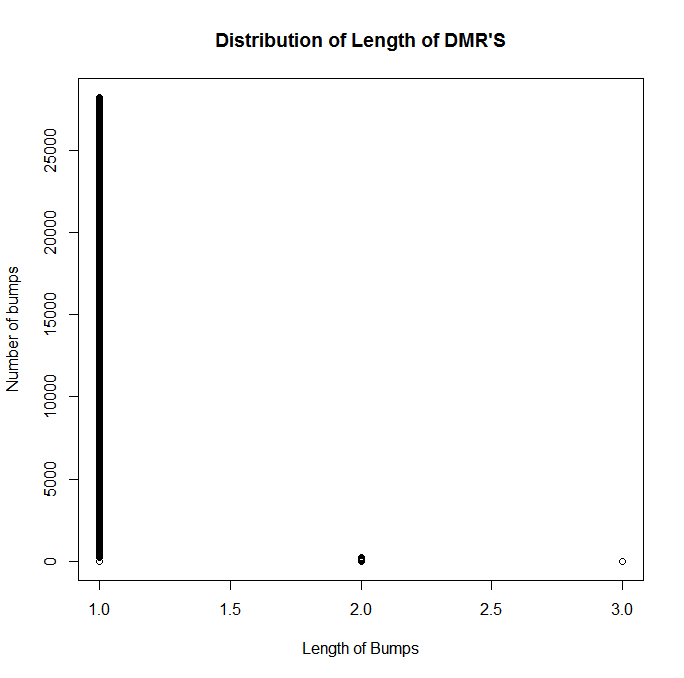
\includegraphics[scale=0.4]{bumpsDistribution.png}

%\begin{verbatim}
%Argument description for bumphunter,
%
%cutoff: 
%
%A numeric value. Values of the estimate of the genomic profile above the cutoff or
%below the negative of the cutoff will be used as candidate regions. It is possible to
%give two separate values (upper and lower bounds). If one value is given, the lower
%bound is minus the value.
%
%pickCutoff: 
%
%Should bumphunter attempt to pick a cutoff using the permutation
%distribution?
%
%\end{verbatim}


%%%%%%%%%%%%%%%%%%%%%%%%%% 
\section*{The Nimblegen Algorithm}
%%%%%%%%%%%%%%%%%%%%%%%%%%

Peaks of enrichment which coincide with methylated regions were found. Peaks near known transcription start sites (TSS) were identified and mapped to overlapping features upto 5000 bp upstream and 1500 downstream in relation to the TSS. In each cell line, the genes which were intersecting among all the samples were identified. To make the two sets independent, all the genes which were identified as common between both cell lines were removed, hence each gene set unique and exclusive for a specific cell line. Both sets of unique and exclusive genes, were ordered by distance from the Transcription start site. 3877 genes were identified in H460 knock-in cell line and 2639 in H460 parent. (Table 2)

\newpage

\captionof{table}{Number of features in each cell line}
\begin{table}[H]
\centering
	\begin{tabular}{|l|l|l|}
	\hline
		Cell line & Feature Track & Number of features \\ \hline
		H460 Knock in & transcription start site & 3877 \\ \hline
		H460 Parent & transcription start site & 2639 \\ \hline
	\end{tabular}
\end{table}


The distribution of the distance from the TSS is also shown for both cell lines. This region encompasses the greater promoter region.

\captionof{table}{Summary of Feature distance from data point}
\begin{table}[H]
\centering
    \begin{tabular}{|l|l|l|l|l|l|l|}
    \hline
     Cell line & Min. & 1st Qu. & Median & Mean & 3rd Qu. &   Max.  \\ \hline
   H460 Knock in  &  -5000  & -3163  & -1503 &  -1599  & 0  &  1500   \\ \hline
   H460 Parent & -4991  & -3500 &  -1900 &  -1756   &    0  &  1499   \\ \hline
    \end{tabular}
\end{table}

\captionof{table}{Distribution of Shortest distance from feature to data point}
\begin{figure}[H]
\centering
\begin{subfigure}{.4\textwidth}
  %\centering
  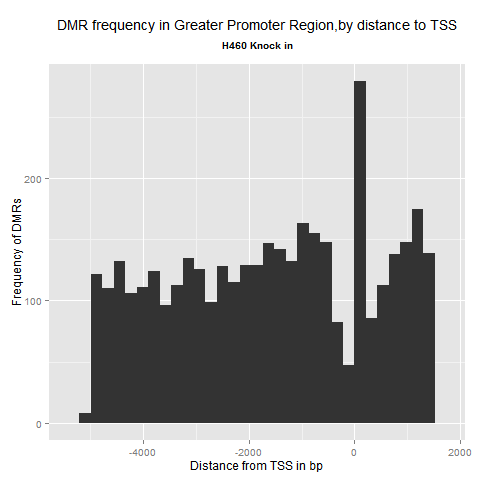
\includegraphics[scale=0.45]{distribution_knocking_annotated_TSS_change.png}
  \caption{H460 knock-in distance from TSS}
  \label{fig:sub1}
\end{subfigure}
\quad
\begin{subfigure}{.4\textwidth}
  %\centering
  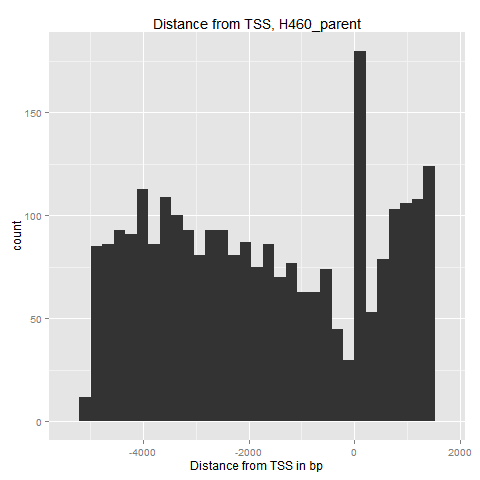
\includegraphics[scale=0.45]{distribution_parent_annotated_TSS_change.png}
  \caption{H460 parent distance from TSS}
  \label{fig:sub2}
\end{subfigure}

\label{fig:test}
\end{figure}



\newpage


%%%%%%%%%%%%%%%%%%%%%%%%%%
\section*{Pathway Comparisons}
%%%%%%%%%%%%%%%%%%%%%%%%%%

Both the list of H460 Knock-in genes and H460 parent genes were compared with a list of selected pathways.

\begin{enumerate}[itemsep=-0.2mm]
\item Cell Cycle                                 
\item Complete Homeobox (HOX) Genes                      
\item Complete Human Inflammatory Response and Autoimmunity 
\item Complete Human Tumor Suppressor Genes              
\item Complete Stem Cell Transcription Factors            
\item Complete Stress and Toxicity                         
\item Cytokine Production                                
\item DNA Repair 
\item Human Epithelial to Mesenchymal Transition (EMT)    
\item Human Notch Signaling Pathway                      
\item Human T-Cell B-Cell Activation Methylation         
\item Human T Helper Cell Differentiation                
\item Human Tumor Suppressor Genes                        
\item Inflammatory Response and Autoimmunity               
\item Polycomb and Trithorax Complexes                     
\item Stem Cell Transcription Factors                    
\item TGF f BMP Signaling Pathway                          
\item Toll-Like Receptor Signaling Pathway               
\item WNT Signaling Pathway                              
\end{enumerate}

Genes which belong to these pathways matched with the H460 knock-in genes and the H460 parent genes are shown graphically to represent the frequency. The H460 knock-in genes have 189 genes in common with the pathways (partially listed in Table 5)and H460 parent genes have  71 genes in pathways(Table 6). 
.The following tables shows you the pathways and the genes along with gene description. Supplemental tables have links to the full results.

\newpage

\captionof{table}{H460 Knock-in gene with corresponding pathways}

\begin{table}[H]
\resizebox{\columnwidth}{!}{
\begin{tabular}{|l|l|l|}
\hline
{\bf name}    & {\bf description}  & {\bf pathway}                                                  \\
\hline
BRCA1   & breast cancer 1, early onset                                                                                   & Cell\_Cycle                                              \\
CCNF    & cyclin F                                                                                                       & Cell\_Cycle                                              \\
RAD9A   & RAD9 homolog A (S. pombe)                                                                                      & Cell\_Cycle                                              \\
TP53    & tumor protein p53                                                                                              & Cell\_Cycle                                              \\
ALX1    & ALX homeobox 1                                                                                                 & Complete\_Homeobox\_(HOX)\_Genes                         \\
ALX4    & ALX homeobox 4                                                                                                 & Complete\_Homeobox\_(HOX)\_Genes                         \\
CDX2    & caudal type homeobox 2                                                                                         & Complete\_Homeobox\_(HOX)\_Genes                         \\
DLX1    & distal-less homeobox 1                                                                                         & Complete\_Homeobox\_(HOX)\_Genes                         \\
DLX5    & distal-less homeobox 5                                                                                         & Complete\_Homeobox\_(HOX)\_Genes                         \\
DLX6    & distal-less homeobox 6                                                                                         & Complete\_Homeobox\_(HOX)\_Genes                         \\
EMX1    & empty spiracles homeobox 1                                                                                     & Complete\_Homeobox\_(HOX)\_Genes                         \\
EN1     & engrailed homeobox 1                                                                                           & Complete\_Homeobox\_(HOX)\_Genes                         \\
HOXA11  & homeobox A11                                                                                                   & Complete\_Homeobox\_(HOX)\_Genes                         \\
HOXA13  & homeobox A13                                                                                                   & Complete\_Homeobox\_(HOX)\_Genes                         \\
HOXA2   & homeobox A2                                                                                                    & Complete\_Homeobox\_(HOX)\_Genes                         \\
HOXA4   & homeobox A4                                                                                                    & Complete\_Homeobox\_(HOX)\_Genes                         \\
HOXA5   & homeobox A5                                                                                                    & Complete\_Homeobox\_(HOX)\_Genes                         \\
HOXA7   & homeobox A7                                                                                                    & Complete\_Homeobox\_(HOX)\_Genes                         \\
HOXA9   & homeobox A9                                                                                                    & Complete\_Homeobox\_(HOX)\_Genes                         \\
HOXB2   & homeobox B2                                                                                                    & Complete\_Homeobox\_(HOX)\_Genes                         \\
HOXB3   & homeobox B3                                                                                                    & Complete\_Homeobox\_(HOX)\_Genes                         \\
HOXB4   & homeobox B4                                                                                                    & Complete\_Homeobox\_(HOX)\_Genes                         \\
HOXB6   & homeobox B6                                                                                                    & Complete\_Homeobox\_(HOX)\_Genes                         \\
HOXB7   & homeobox B7                                                                                                    & Complete\_Homeobox\_(HOX)\_Genes                         \\
HOXB8   & homeobox B8                                                                                                    & Complete\_Homeobox\_(HOX)\_Genes                         \\
HOXC10  & homeobox C10                                                                                                   & Complete\_Homeobox\_(HOX)\_Genes                         \\
HOXC11  & homeobox C11                                                                                                   & Complete\_Homeobox\_(HOX)\_Genes                         \\
HOXC12  & homeobox C12                                                                                                   & Complete\_Homeobox\_(HOX)\_Genes                         \\
HOXC13  & homeobox C13                                                                                                   & Complete\_Homeobox\_(HOX)\_Genes                         \\
HOXD1   & homeobox D1                                                                                                    & Complete\_Homeobox\_(HOX)\_Genes                         \\
HOXD10  & homeobox D10                                                                                                   & Complete\_Homeobox\_(HOX)\_Genes                         \\
HOXD11  & homeobox D11                                                                                                   & Complete\_Homeobox\_(HOX)\_Genes                         \\
HOXD12  & homeobox D12                                                                                                   & Complete\_Homeobox\_(HOX)\_Genes                         \\
HOXD3   & homeobox D3                                                                                                    & Complete\_Homeobox\_(HOX)\_Genes                         \\
HOXD9   & homeobox D9                                                                                                    & Complete\_Homeobox\_(HOX)\_Genes                         \\
ISL1    & ISL LIM homeobox 1                                                                                             & Complete\_Homeobox\_(HOX)\_Genes                         \\
LBX1    & ladybird homeobox 1                                                                                            & Complete\_Homeobox\_(HOX)\_Genes                         \\
LBX2    & ladybird homeobox 2                                                                                            & Complete\_Homeobox\_(HOX)\_Genes                         \\
MIXL1   & Mix1 homeobox-like 1 (Xenopus laevis)                                                                          & Complete\_Homeobox\_(HOX)\_Genes                         \\
MSX2    & msh homeobox 2                                                                                                 & Complete\_Homeobox\_(HOX)\_Genes                         \\
PHOX2A  & paired-like homeobox 2a                                                                                        & Complete\_Homeobox\_(HOX)\_Genes                         \\
PHOX2B  & paired-like homeobox 2b                                                                                        & Complete\_Homeobox\_(HOX)\_Genes                         \\
PITX3   & paired-like homeodomain 3                                                                                      & Complete\_Homeobox\_(HOX)\_Genes                         \\
BCL6    & B-cell CLL/lymphoma 6                                                                                          & Complete\_Human\_Inflammatory\_Response\_\&\_Autoimmunity \\
CD276   & CD276 molecule                                                                                                 & Complete\_Human\_Inflammatory\_Response\_\&\_Autoimmunity \\
CXCL5   & chemokine (C-X-C motif) ligand 5                                                                               & Complete\_Human\_Inflammatory\_Response\_\&\_Autoimmunity \\
IL10RB  & interleukin 10 receptor, beta                                                                                  & Complete\_Human\_Inflammatory\_Response\_\&\_Autoimmunity \\
IL17RA  & interleukin 17 receptor A                                                                                      & Complete\_Human\_Inflammatory\_Response\_\&\_Autoimmunity \\
IL4R    & interleukin 4 receptor                                                                                         & Complete\_Human\_Inflammatory\_Response\_\&\_Autoimmunity \\
IL6ST   & interleukin 6 signal transducer (gp130, oncostatin M receptor)                                                 & Complete\_Human\_Inflammatory\_Response\_\&\_Autoimmunity \\
INHBA   & inhibin, beta A                                                                                                & Complete\_Human\_Inflammatory\_Response\_\&\_Autoimmunity \\
IRF1    & interferon regulatory factor 1                                                                                 & Complete\_Human\_Inflammatory\_Response\_\&\_Autoimmunity \\
LTB4R   & leukotriene B4 receptor                                                                                        & Complete\_Human\_Inflammatory\_Response\_\&\_Autoimmunity \\
NOD1    & nucleotide-binding oligomerization domain containing 1                                                         & Complete\_Human\_Inflammatory\_Response\_\&\_Autoimmunity \\
PAX1    & paired box 1                                                                                                   & Complete\_Human\_Inflammatory\_Response\_\&\_Autoimmunity \\
RELA    & v-rel reticuloendotheliosis viral oncogene homolog A (avian)                                                   & Complete\_Human\_Inflammatory\_Response\_\&\_Autoimmunity \\
S1PR3   & sphingosine-1-phosphate receptor 3                                                                             & Complete\_Human\_Inflammatory\_Response\_\&\_Autoimmunity \\
SOCS1   & suppressor of cytokine signaling 1                                                                             & Complete\_Human\_Inflammatory\_Response\_\&\_Autoimmunity \\
TH1L    & TH1-like (Drosophila)                                                                                          & Complete\_Human\_Inflammatory\_Response\_\&\_Autoimmunity \\
TIRAP   & toll-interleukin 1 receptor (TIR) domain containing adaptor protein                                            & Complete\_Human\_Inflammatory\_Response\_\&\_Autoimmunity \\
\hline
\end{tabular}}
\end{table}

\newpage

\captionof{table}{H460 parent gene with corresponding pathways }
\begin{table}[H]
\resizebox{\columnwidth}{!}{
\begin{tabular}{|l|l|l|}
\hline
\textbf{name} & \textbf{description}                                                                                      & \textbf{pathway}                                    \\ \hline 
BRCA2         & breast cancer 2  early onset                                                                              & Cell\_Cycle                                                \\ 
CCNE1         & cyclin E1                                                                                                 & Cell\_Cycle                                                \\ 
MRE11A        & MRE11 meiotic recombination 11 homolog A (S. cerevisiae)                                                  & Cell\_Cycle                                                \\ 
HOPX          & HOP homeobox                                                                                              & Complete\_Homeobox\_(HOX)\_Genes                           \\ 
MKX           & mohawk homeobox                                                                                           & Complete\_Homeobox\_(HOX)\_Genes                           \\ 
SIX6          & SIX homeobox 6                                                                                            & Complete\_Homeobox\_(HOX)\_Genes                           \\
ATF2          & activating transcription factor 2                                                                         & Complete\_Human\_Inflammatory\_Response\_and\_Autoimmunity \\ 
CD274         & CD274 molecule                                                                                            & Complete\_Human\_Inflammatory\_Response\_and\_Autoimmunity \\ 
CXCL1         & chemokine (C-X-C motif) ligand 1 (melanoma growth stimulating activity  alpha)                            & Complete\_Human\_Inflammatory\_Response\_and\_Autoimmunity \\ 
IL12A         & interleukin 12A (natural killer cell stimulatory factor 1  cytotoxic lymphocyte maturation factor 1  p35) & Complete\_Human\_Inflammatory\_Response\_and\_Autoimmunity \\ 
IL12B         & interleukin 12B (natural killer cell stimulatory factor 2  cytotoxic lymphocyte maturation factor 2  p40) & Complete\_Human\_Inflammatory\_Response\_and\_Autoimmunity \\ 
IL15          & interleukin 15                                                                                            & Complete\_Human\_Inflammatory\_Response\_and\_Autoimmunity \\ 
NFKB1         & nuclear factor of kappa light polypeptide gene enhancer in B-cells 1                                      & Complete\_Human\_Inflammatory\_Response\_and\_Autoimmunity \\ 
RIPK2         & receptor-interacting serine-threonine kinase 2                                                            & Complete\_Human\_Inflammatory\_Response\_and\_Autoimmunity \\ 
TLR2          & toll-like receptor 2                                                                                      & Complete\_Human\_Inflammatory\_Response\_and\_Autoimmunity \\ 
BRCA2         & breast cancer 2  early onset                                                                              & Complete\_Human\_Tumor\_Suppressor\_Genes                  \\ 
CDKN2A        & cyclin-dependent kinase inhibitor 2A (melanoma  p16  inhibits CDK4)                                       & Complete\_Human\_Tumor\_Suppressor\_Genes                  \\ 
ING1          & inhibitor of growth family  member 1                                                                      & Complete\_Human\_Tumor\_Suppressor\_Genes                  \\ 
MDM2          & Mdm2 p53 binding protein homolog (mouse)                                                                  & Complete\_Human\_Tumor\_Suppressor\_Genes                  \\ 
NFKB1         & nuclear factor of kappa light polypeptide gene enhancer in B-cells 1                                      & Complete\_Human\_Tumor\_Suppressor\_Genes                  \\ 
AR            & androgen receptor                                                                                         & Complete\_Stem\_Cell\_Transcription\_Factors               \\ 
DACH1         & dachshund homolog 1 (Drosophila)                                                                          & Complete\_Stem\_Cell\_Transcription\_Factors               \\ 
NFYA          & nuclear transcription factor Y  alpha                                                                     & Complete\_Stem\_Cell\_Transcription\_Factors               \\ 
PCNA          & proliferating cell nuclear antigen                                                                        & Complete\_Stem\_Cell\_Transcription\_Factors               \\ 
RUNX2         & runt-related transcription factor 2                                                                       & Complete\_Stem\_Cell\_Transcription\_Factors               \\ 
SMAD2         & SMAD family member 2                                                                                      & Complete\_Stem\_Cell\_Transcription\_Factors               \\ 
SOX2          & SRY (sex determining region Y)-box 2                                                                      & Complete\_Stem\_Cell\_Transcription\_Factors               \\ 
WRN           & Werner syndrome  RecQ helicase-like                                                                       & Complete\_Stem\_Cell\_Transcription\_Factors               \\ 
ZFPM2         & zinc finger protein  multitype 2                                                                          & Complete\_Stem\_Cell\_Transcription\_Factors               \\ 
DNAJB9        & DnaJ (Hsp40) homolog  subfamily B  member 9                                                               & Complete\_Stress\_and\_Toxicity                            \\ 
MDM2          & Mdm2 p53 binding protein homolog (mouse)                                                                  & Complete\_Stress\_and\_Toxicity                            \\ 
MRE11A        & MRE11 meiotic recombination 11 homolog A (S. cerevisiae)                                                  & Complete\_Stress\_and\_Toxicity                            \\ 
NFKB1         & nuclear factor of kappa light polypeptide gene enhancer in B-cells 1                                      & Complete\_Stress\_and\_Toxicity                            \\ 
PCNA          & proliferating cell nuclear antigen                                                                        & Complete\_Stress\_and\_Toxicity                            \\ 
RAD17         & RAD17 homolog (S. pombe)                                                                                  & Complete\_Stress\_and\_Toxicity                            \\ 
IL12A         & interleukin 12A (natural killer cell stimulatory factor 1  cytotoxic lymphocyte maturation factor 1  p35) & Cytokine\_Production                                       \\ 
TLR2          & toll-like receptor 2                                                                                      & Cytokine\_Production                                       \\ 
BRCA2         & breast cancer 2  early onset                                                                              & DNA\_Repair                                                \\ 
MLH3          & mutL homolog 3 (E. coli)                                                                                  & DNA\_Repair                                                \\ 
MRE11A        & MRE11 meiotic recombination 11 homolog A (S. cerevisiae)                                                  & DNA\_Repair                                                \\ 
CTNNAL1       & catenin (cadherin-associated protein)  alpha-like 1                                                       & Human\_Epithelial\_to\_Mesenchymal\_Transition\_(EMT)      \\ 
DSP           & desmoplakin                                                                                               & Human\_Epithelial\_to\_Mesenchymal\_Transition\_(EMT)      \\ 
TGIF1         & TGFB-induced factor homeobox 1                                                                            & Human\_Epithelial\_to\_Mesenchymal\_Transition\_(EMT)      \\ 
YES1          & v-yes-1 Yamaguchi sarcoma viral oncogene homolog 1                                                        & Human\_Epithelial\_to\_Mesenchymal\_Transition\_(EMT)      \\ 
HDAC2         & histone deacetylase 2                                                                                     & Human\_Notch\_Signaling\_Pathway                           \\ 
CD274         & CD274 molecule                                                                                            & Human\_T-Cell\_B-Cell\_Activation\_Methylation             \\ 
IL12A         & interleukin 12A (natural killer cell stimulatory factor 1  cytotoxic lymphocyte maturation factor 1  p35) & Human\_T-Cell\_B-Cell\_Activation\_Methylation             \\ 
RIPK2         & receptor-interacting serine-threonine kinase 2                                                            & Human\_T-Cell\_B-Cell\_Activation\_Methylation             \\ 
IRF8          & interferon regulatory factor 8                                                                            & Human\_T\_Helper\_Cell\_Differentiation                    \\ 
PERP          & PERP  TP53 apoptosis effector                                                                             & Human\_T\_Helper\_Cell\_Differentiation                    \\ 
TGIF1         & TGFB-induced factor homeobox 1                                                                            & Human\_T\_Helper\_Cell\_Differentiation                    \\ 
TNFSF11       & tumor necrosis factor (ligand) superfamily  member 11                                                     & Human\_T\_Helper\_Cell\_Differentiation                    \\ \hline
\end{tabular}}
\end{table}



%%Table 7 describes the number of features in each cell line. 
%%
%%\captionof{table}{Number of features in each cell line with extended window}
%\begin{table}[H]
%\centering
%	\begin{tabular}{|l|l|l|}
%	\hline
%		Cell line & Feature Track & Number of features \\ \hline
%		H460 Knock in & transcription start site & 3877 \\ \hline
%		H460 Parent & transcription start site & 2639 \\ \hline
%	\end{tabular}
%\end{table}



%%%%%%%%%%%%%%%%%%%%%%%%%%
\section*{R-packages Used}
%%%%%%%%%%%%%%%%%%%%%%%%%%

List of R-packages used for analysis:
\begin{enumerate}[itemsep=-0.2mm]

\item Charm

\item Bioconductor

\item BiocGenerics

\item plyr

\item RCircos

%\item 

\end{enumerate}




%%%%%%%%%%%%%%%%%%%%%%%%%%
\section*{References}  
%%%%%%%%%%%%%%%%%%%%%%%%%%
\begin{enumerate}


	\item  Aryee MJ et al., Accurate genome-scale percentage DNA methylation estimates
	  from microarray data, Biostatistics (2011) 12(2): 197-210 	

	\item  Seth Falcon, Benilton Carvalho with contributions by Vince Carey, Matt
	  Settles and Kristof de Beuf. pdInfoBuilder: Platform Design Information
	  Package Builder. R package version 1.24.0.
	
	\item   Rafael A. Irizarry, Martin Aryee, Hector Corrada Bravo, Kasper D. Hansen and	Harris A. Jaffee (). bumphunter: Bump Hunter. R package version 1.0.0.
		
	\item RCircos: an R package for Circos 2D track plots
	


	\item \href{http://www.ncbi.nlm.nih.gov/pmc/articles/PMC2336799/}{Irizarry RA, Ladd-Acosta C, Carvalho B, et al. Comprehensive high-throughput arrays for relative methylation (CHARM) Genome Res. 2008;18(5):780–790.} 
	
	\item Martin J. Aryee, Zhijin Wu, Christine Ladd-Acosta, Brian Herb, Andrew P.
Feinberg, Srinivasan Yegnasubramanian, and Rafael A. Irizarry. Accurate
genome-scale percentage dna methylation estimates from microarray data.
Biostatistics, 12(2):197-210, 2011.

\end{enumerate}



%%%%%%%%%%%%%%%%%%%%%%%%%%%%%%%
\section*{Supplementary Tables}  
%%%%%%%%%%%%%%%%%%%%%%%%%%%%%%%

The results of the pathway analysis and their links are provided.

\begin{enumerate}

	\item \href{https://app.box.com/s/7xr01qkv3xx41oo5izew}{H460 knock-in genes with corresponding pathways, with changed cutoff of -5000 to +1500.(https://app.box.com/s/7xr01qkv3xx41oo5izew)} 
%	
	\item \href{https://app.box.com/s/pu0n89gusqlf1umjwwhh}{H460 parent genes with corresponding pathways,  with changed cutoff of -5000 to +1500.(https://app.box.com/s/pu0n89gusqlf1umjwwhh)}
\end{enumerate}

 

 
\end{document}


